\documentclass[submit]{../harvardml}
\usepackage{../common}

\assignment{Homework \#5}
\duedate{April 19, 2026 at 11:59pm}

\usepackage[OT1]{fontenc}
\usepackage[colorlinks,citecolor=blue,urlcolor=blue]{hyperref}
\usepackage{graphicx}
\usepackage{subcaption}
\usepackage{amsmath}
\usepackage{amssymb}
\usepackage{booktabs}
\usepackage{float}
\usepackage{framed}
\usepackage{xcolor}
\usepackage{enumitem}
\graphicspath{{img_output/}}

\newenvironment{solution}{%
    \vspace{2mm}\color{blue}\noindent\textbf{Solution}:\ }
{}

\begin{document}

\begin{center}
{\Large Clustering, PCA, SSL}\\
\end{center}

\subsection*{Overview}
This homework contains four problems:
\begin{enumerate}[leftmargin=*]
    \item SimCLR and contrastive learning.
    \item GANs and the Jensen--Shannon divergence interpretation.
    \item K-means and hierarchical agglomerative clustering on handwritten digits.
    \item PCA on MNIST.
\end{enumerate}
The coding portions are consolidated in \texttt{hw5\_release.ipynb}. The clustering and PCA plots used below are stored in \texttt{img\_output/}.

\subsection*{Resources and Submission Instructions}
Please type your answers after the corresponding problems using this \LaTeX\ template, and start each main problem on a new page.

Please submit the writeup PDF to the Gradescope assignment \texttt{HW5}. Remember to assign pages for each question. \textbf{You must include any plots in your writeup PDF.} Please submit your \LaTeX\ file and code files to the Gradescope assignment \texttt{HW5 - Supplemental}. Your files should be named in the same way as we provide them in the repository, for example \texttt{hw5\_release.tex} and \texttt{hw5\_release.ipynb}.

\begin{problem}[Contrastive Learning]
In this problem we study SimCLR, a self-supervised learning framework that learns visual representations without labels by training a network to identify which data augmentations came from the same image.

This problem mixes short written questions with an implementation scaffold. In the notebook, the SimCLR section is organized in the same order as the written prompt: encoder backbone, projection head, NT-Xent loss, verification, pre-training, and linear evaluation.

\begin{enumerate}[leftmargin=*]
\item \textbf{SimCLR and the NT-Xent loss.}

The SimCLR pipeline works as follows. Given a minibatch of \(N\) images, each image \(x_k\) is augmented twice, producing a positive pair \((\tilde{x}_{2k-1}, \tilde{x}_{2k})\). This yields \(2N\) augmented views total. Each view is passed through an encoder \(f\) and a projection head \(g\) to produce normalized embeddings
\[
\mathbf{z}_i = \frac{g(f(\tilde{x}_i))}{\|g(f(\tilde{x}_i))\|}.
\]
For a positive pair \((i,j)\), the NT-Xent loss is
\[
\ell(i,j) = -\log \frac{\exp(\mathbf{z}_i^\top \mathbf{z}_j / \tau)}{\sum_{k=1,\,k\neq i}^{2N} \exp(\mathbf{z}_i^\top \mathbf{z}_k / \tau)},
\]
where \(\tau > 0\) is a temperature parameter.

\begin{enumerate}[label=(\alph*)]
    \item Show that \(\ell(i,j)\) is equivalent to the cross-entropy loss of a \((2N-1)\)-way classification problem in which the positive partner \(j\) is the correct class and the remaining \(2N-2\) embeddings are negatives.
    \item Consider the softmax weight assigned to a negative sample \(k \neq j\):
    \[
    w_k = \frac{\exp(\mathbf{z}_i^\top \mathbf{z}_k / \tau)}{\sum_{m=1,\,m\neq i}^{2N} \exp(\mathbf{z}_i^\top \mathbf{z}_m / \tau)}.
    \]
    Explain what happens as \(\tau \to 0^+\), what happens as \(\tau \to \infty\), and why an intermediate temperature is preferred in practice.
\end{enumerate}

\item \textbf{Representation collapse and augmentations.}
\begin{enumerate}[label=(\alph*)]
    \item Compute \(\ell(i,j)\) under the collapse solution \(f(x)=\mathbf c\), where \(\mathbf c\) is a constant unit vector and therefore every pairwise similarity is \(1\).
    \item Explain intuitively why the encoder representation \(\mathbf h=f(x)\) is often more useful downstream than the projection-head output \(\mathbf z=g(f(x))\).
    \item Discuss the effect of overly aggressive augmentations and overly weak augmentations on the learned representation.
\end{enumerate}

\item \textbf{Implementing SimCLR components (code).}
In the notebook, implement:
\begin{enumerate}[label=(\alph*)]
    \item a two-layer projection head \(\mathrm{Linear} \to \mathrm{ReLU} \to \mathrm{Linear}\), and
    \item the NT-Xent loss for two batches of projected views.
\end{enumerate}
The intended implementation flow is:
\begin{enumerate}[label=(\roman*)]
    \item \(\ell_2\)-normalize the representations,
    \item concatenate them into a \(2N \times d_z\) matrix,
    \item compute the \(2N \times 2N\) cosine-similarity matrix scaled by \(1/\tau\),
    \item mask self-similarities,
    \item identify the positive-pair index for each view, and
    \item compute cross-entropy loss using the positive index as the target.
\end{enumerate}
The corresponding notebook cells are grouped under the SimCLR headings
\texttt{Projection Head}, \texttt{NT-Xent Loss}, and
\texttt{Run Test Cases}.

\item \textbf{SimCLR training and linear evaluation (code).}
Use the provided training scaffold to:
\begin{enumerate}[label=(\alph*)]
    \item pre-train the encoder and projection head on FashionMNIST without labels,
    \item freeze the encoder and run linear evaluation on top of the learned features, and
    \item compare the resulting linear-evaluation accuracy against a supervised baseline with the same encoder architecture.
\end{enumerate}
In the notebook, these correspond to the sections
\texttt{Data Loading and Augmentations},
\texttt{SimCLR Pre-training},
\texttt{Linear Evaluation}, and
\texttt{Supervised Baseline}.
\end{enumerate}
\end{problem}

\newpage

\begin{solution}

\textbf{1(a).} The cross entropy loss for a $(2N{-}1)$ way classification problem with logits $\{s_k\}_{k \neq i}$ and true class $j$ is:
\[
L_{\mathrm{CE}} = -\log \frac{\exp(s_j)}{\sum_{k=1,\,k \neq i}^{2N} \exp(s_k)}
\]
Setting the logits to be the temperature scaled cosine similarities $s_k = z_i^\top z_k / \tau$ for all $k \neq i$, we obtain exactly the NT-Xent loss $\ell(i,j)$. The denominator sums over the $2N - 1$ indices $k \neq i$, so the softmax has $2N - 1$ classes. The numerator selects the positive partner $j$ as the correct class while the remaining $2N - 2$ embeddings serve as negatives. Thus $\ell(i,j)$ is equivalent to cross entropy over a $(2N{-}1)$ way classification where the target is the positive pair index $j$.

\textbf{1(b).} As $\tau \to 0^+$, the softmax sharpens and $w_k$ concentrates all mass on the negative with the highest similarity to $z_i$. In the limit, only the single hardest negative receives a nonzero weight. As $\tau \to \infty$, the exponents $z_i^\top z_k / \tau \to 0$ for all $k$, so $w_k \to 1/(2N-1)$ uniformly. The loss approaches $\log(2N-1)$ regardless of the embedding geometry, providing no useful gradient signal for distinguishing positives from negatives. An intermediate temperature is preferred because it allows the loss to focus learning on moderately hard negatives, those that are somewhat similar to the anchor, without either ignoring easy negatives entirely (low $\tau$) or treating all negatives as equally uninformative (high $\tau$).

\textbf{2(a).} Under the collapse solution $f(x) = c$ with $\|c\| = 1$, every pairwise cosine similarity equals $1$. Thus:
\[
\ell(i,j) = -\log \frac{\exp(1/\tau)}{\sum_{k \neq i}^{2N} \exp(1/\tau)} = -\log \frac{\exp(1/\tau)}{(2N-1)\exp(1/\tau)} = \log(2N-1)
\]
This is the maximum entropy baseline, the loss treats the positive pair as no more similar than any negative, so the contrastive objective does not decrease. The collapse solution is therefore not a minimizer of the NT-Xent loss.

\textbf{2(b).} The projection head $g$ is trained to produce embeddings that are invariant to augmentations, so it discards information about augmentation specific details (for example crop position, rotation angle) that are irrelevant to the contrastive task. The encoder representation $h = f(x)$ retains this richer information, making it more useful for diverse downstream tasks that may require features the contrastive objective does not explicitly preserve.

\textbf{2(c).} Overly aggressive augmentations destroy class discriminative content, so positive pairs from the same image may share nothing semantically. The encoder then learns low level statistical regularities rather than meaningful class structure. Overly weak augmentations make the contrastive task trivial, positive pairs are nearly identical, so the encoder can succeed by memorizing superficial pixel patterns without learning invariant, transferable representations. A good augmentation distribution forces the encoder to capture semantic similarity while discarding unimportant variation.

\textbf{3.} Implemented in \texttt{hw5\_release.ipynb}.

\textbf{4.} Implemented in \texttt{hw5\_release.ipynb}. The SimCLR pre training loss over epochs is shown below, followed by the linear evaluation accuracy comparison:

\begin{center}
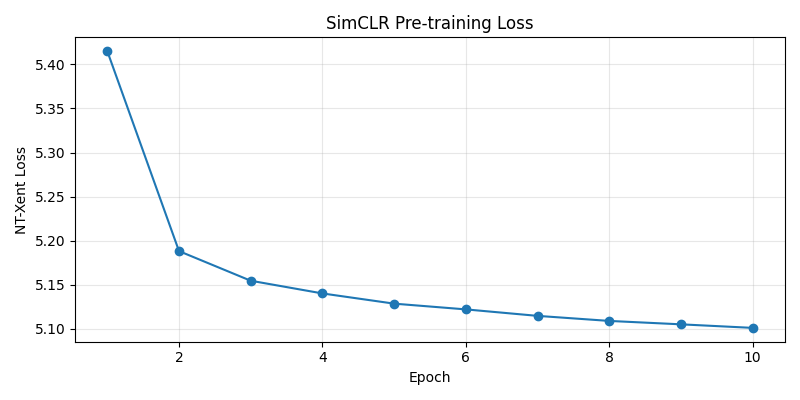
\includegraphics[width=0.7\textwidth]{simclr_loss.png}
\end{center}

\begin{center}
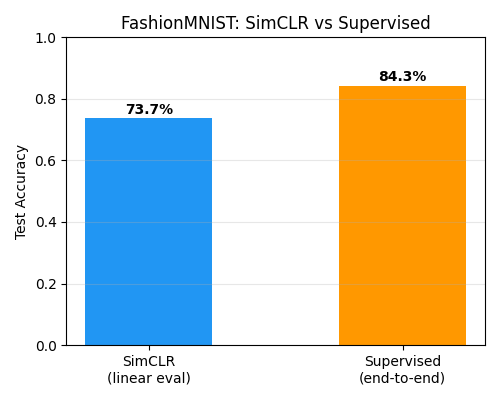
\includegraphics[width=0.5\textwidth]{simclr_comparison.png}
\end{center}

\end{solution}

\newpage

\begin{problem}[GANs]
Consider the original minimax GAN objective
\[
\min_G \max_D V(D,G) = \mathbb E_{x\sim p_{\mathrm{data}}}[\log D(x)] + \mathbb E_{z\sim p_z}[\log(1-D(G(z)))] .
\]
Let \(p_g\) denote the distribution induced by \(x = G(z)\).

This problem has both a written component and a coding component.

\begin{itemize}[leftmargin=*]
    \item \textbf{Written work:} derive the optimal discriminator, rewrite the GAN objective in terms of the Jensen--Shannon divergence, and explain the resulting training objectives in words and equations.
    \item \textbf{Code work:} implement the practical GAN training loop in the notebook by defining the generator and discriminator, implementing the discriminator and generator losses, and alternating the two updates during training.
\end{itemize}

The GAN notebook section is deliberately split into small cells so that the mathematical objectives and the alternating training logic are easy to match to the code. The intended order is data setup, model definitions, loss definitions, one-epoch training logic, and then the multi-epoch training loop.

\begin{enumerate}[leftmargin=*]
    \item \textbf{Interpreting GANs as Jensen--Shannon divergence (written).}
    Assume \(G\) is fixed.
    \begin{enumerate}[label=(\alph*)]
        \item Derive the optimal discriminator \(D^*(x)\) in terms of \(p_{\mathrm{data}}(x)\) and \(p_g(x)\).
        \item Substitute \(D^*(x)\) back into the GAN objective and show that the result can be written as a constant plus a Jensen--Shannon divergence term.
        \item Explain, in words, what this means for what the generator is trying to do.
    \end{enumerate}
    \item \textbf{From derivation to training algorithm (written).}
    \begin{enumerate}[label=(\alph*)]
        \item Write the discriminator objective.
        \item Write the generator objective.
        \item Describe the alternating training loop used in practice.
    \end{enumerate}
    \item \textbf{GAN implementation (code).}
    In the notebook, complete the practical GAN scaffold by:
    \begin{enumerate}[label=(\alph*)]
        \item defining the generator and discriminator networks,
        \item implementing the discriminator loss on real and fake batches,
        \item implementing the generator loss,
        \item writing the alternating update logic for one epoch of training, and
        \item training for multiple epochs and visualizing generated samples.
    \end{enumerate}
    In \texttt{hw5\_release.ipynb}, these correspond to the GAN section cells for model setup, loss definitions, \texttt{train\_one\_epoch}, and the final training loop.
\end{enumerate}
\end{problem}

\newpage

\begin{solution}

\textbf{1(a).} For fixed $G$, we maximize $V(D,G)$ pointwise over $D(x)$. At each $x$, the integrand is:
\[
h(D) = p_{\mathrm{data}}(x)\log D(x) + p_g(x)\log(1 - D(x))
\]
Taking the derivative and setting it to zero:
\[
\frac{p_{\mathrm{data}}(x)}{D(x)} - \frac{p_g(x)}{1 - D(x)} = 0 \implies D^*(x) = \frac{p_{\mathrm{data}}(x)}{p_{\mathrm{data}}(x) + p_g(x)}
\]

\textbf{1(b).} Substituting $D^*$ back into the objective:
\begin{align*}
V(D^*, G) &= \mathbb{E}_{x \sim p_{\mathrm{data}}}\!\left[\log \frac{p_{\mathrm{data}}(x)}{p_{\mathrm{data}}(x) + p_g(x)}\right] + \mathbb{E}_{x \sim p_g}\!\left[\log \frac{p_g(x)}{p_{\mathrm{data}}(x) + p_g(x)}\right]
\end{align*}
Let $m(x) = \tfrac{1}{2}(p_{\mathrm{data}}(x) + p_g(x))$. Then we can write:
\begin{align*}
V(D^*, G) &= \mathbb{E}_{p_{\mathrm{data}}}\!\left[\log \frac{p_{\mathrm{data}}}{2m}\right] + \mathbb{E}_{p_g}\!\left[\log \frac{p_g}{2m}\right] \\
&= \mathrm{KL}(p_{\mathrm{data}} \| m) + \mathrm{KL}(p_g \| m) - 2\log 2 \\
&= 2\,\mathrm{JSD}(p_{\mathrm{data}} \| p_g) - \log 4
\end{align*}

\textbf{1(c).} Since $V(D^*,G) = 2\,\mathrm{JSD}(p_{\mathrm{data}} \| p_g) - \log 4$ and $\mathrm{JSD} \geq 0$ with equality iff $p_{\mathrm{data}} = p_g$, the generator minimizes the Jensen--Shannon divergence between the generated distribution and the true data distribution. In other words, $G$ is trying to make $p_g$ match $p_{\mathrm{data}}$ as closely as possible.

\textbf{2(a).} The discriminator objective is:
\[
\max_D \; \mathbb{E}_{x \sim p_{\mathrm{data}}}[\log D(x)] + \mathbb{E}_{z \sim p_z}[\log(1 - D(G(z)))]
\]

\textbf{2(b).} In practice, we use the non saturating generator objective:
\[
\max_G \; \mathbb{E}_{z \sim p_z}[\log D(G(z))].
\]
This avoids the vanishing gradient problem of the original $\min_G \mathbb{E}_{z}[\log(1 - D(G(z)))]$ formulation when $D$ is confident.

\textbf{2(c).} The alternating training procedure for each mini batch is:
\begin{enumerate}
\item Sample a batch of real images $\{x_i\}$ and latent vectors $\{z_i\}$. Generate fake images $G(z_i)$.
\item Update $D$: compute the discriminator loss on the real batch (target $= 1$) and the detached fake batch (target $= 0$), then take a gradient step on $D$.
\item Update $G$: sample fresh latent vectors, generate new fake images, compute the generator loss (target $= 1$ for the discriminator output on fakes), then take a gradient step on $G$.
\end{enumerate}
The two optimizers alternate. $G$ never sees gradients from the discriminator update on real data, and $D$ never sees gradients flowing back through $G$'s parameters.

\textbf{3.} Implemented in \texttt{hw5\_release.ipynb}. A grid of generated samples after training is shown below:

\begin{center}
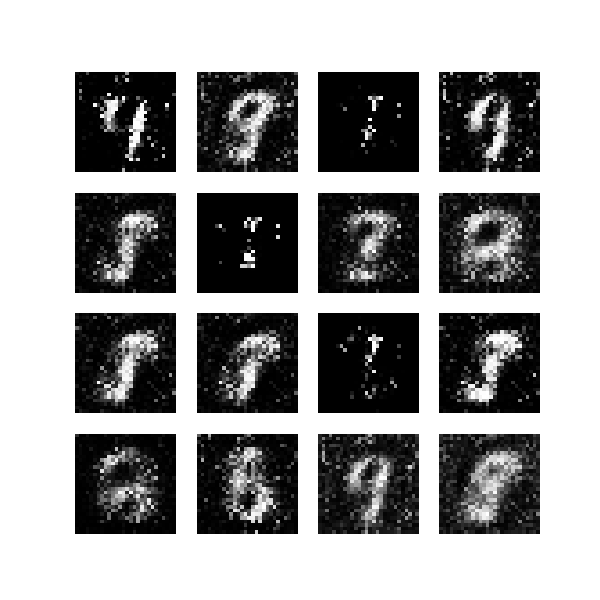
\includegraphics[width=0.5\textwidth]{gan_generated.png}
\end{center}

\end{solution}

\newpage

\begin{problem}[K-Means and HAC]
For this problem, K-means and hierarchical agglomerative clustering are implemented from scratch and applied to handwritten-digit data.

Your job is to implement K-means and HAC on MNIST and test whether these relatively simple algorithms can cluster similar-looking images together. The clustering section of the notebook is organized by subproblem number so that each saved figure can be traced back to the corresponding written prompt.

\begin{enumerate}[leftmargin=*]
    \item The code loads the images into two arrays: \texttt{large\_dataset}, a \(5000 \times 784\) array used for K-means, and \texttt{small\_dataset}, a \(300 \times 784\) array used for HAC. A companion array \texttt{small\_dataset\_labels} is used only for the confusion-matrix comparison. In your code, use the \(\ell_2\) norm (Euclidean distance) as the distance metric.
    \item Starting from a random initialization with \(K=10\), plot the K-means objective function as a function of iteration and verify that it never increases.
    \item For \(K=10\) and three random restarts, display the mean image for each cluster. Present the \(30\) total images in a single plot.
    \item Repeat the previous part after standardizing each pixel to have mean \(0\) and variance \(1\), dividing by \(1\) for any zero-variance pixels. Compare the resulting centroids to the unstandardized case.
    \item Implement HAC for max, min, and centroid linkage. Fit each method to the small dataset and show the mean image for each cluster when there are exactly \(10\) clusters. Comment on crispness and explain why HAC only needs one run.
    \item For each HAC linkage and for one K-means run, plot the number of images in each cluster at the stage where there are \(10\) clusters. Explain what these plots say about max-linkage versus min-linkage behavior.
    \item Using the K-means and HAC assignments on the small dataset, plot the pairwise confusion matrices between the clustering methods. Identify which HAC variant is closest to K-means and explain why.
    \item Discuss whether clustering is a good strategy for digit identification, whether clusters should be expected to match true labels, and what kinds of bad or adversarial data are especially problematic for clustering methods.
\end{enumerate}
\end{problem}

\newpage

\begin{solution}

\textbf{1.} Everything is implemented as described in the problem statement.

\textbf{2.} The K-means objective is plotted as a function of iteration below. By construction, neither the assignment step nor the mean update step can increase this objective, so it is monotonically non increasing:

\begin{center}
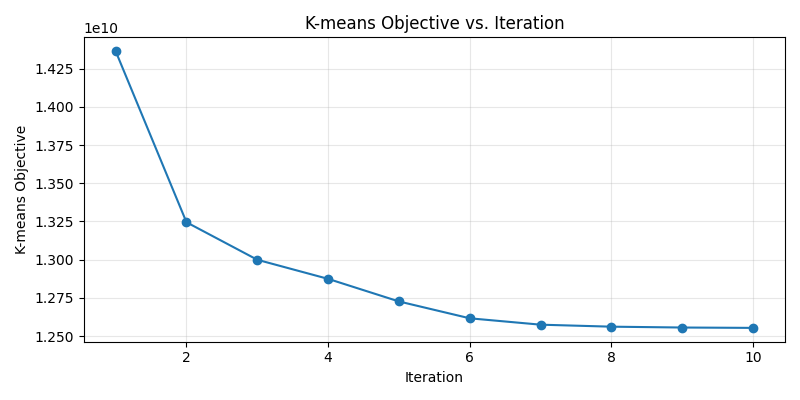
\includegraphics[width=0.6\textwidth]{p2_objective.png}
\end{center}

\textbf{3.} The $10$ cluster mean images across $3$ random restarts are shown below. Different initializations yield different clusterings, but the centroids consistently resemble digit prototypes:

\begin{center}
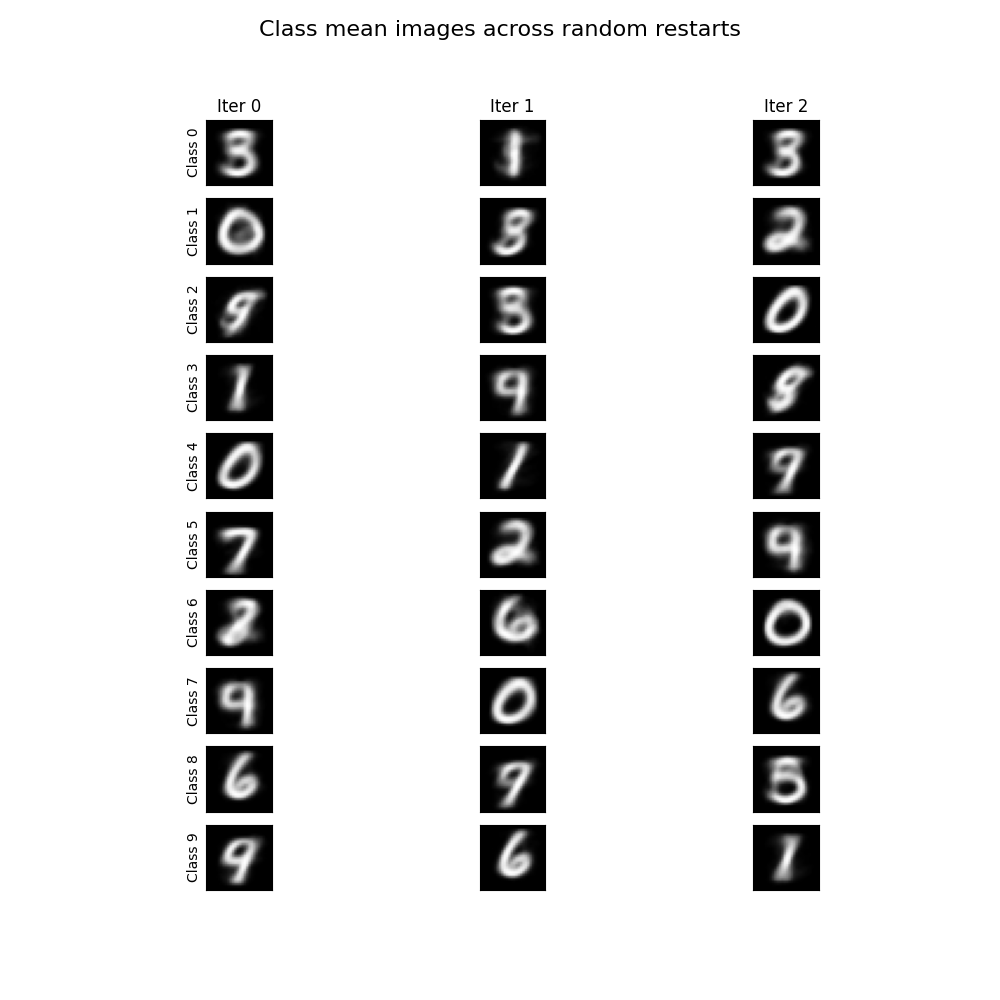
\includegraphics[width=0.85\textwidth]{p2.2.png}
\end{center}

\textbf{4.} After standardizing each pixel to have mean $0$ and variance $1$, the resulting centroids emphasize digit outlines and edge structure more than raw stroke intensity. Standardization upweights low variance pixels, typically at the borders of the digit region, causing the algorithm to pay more attention to the shape of the boundary rather than the thickness of the central strokes. Images are shown below:

\begin{center}
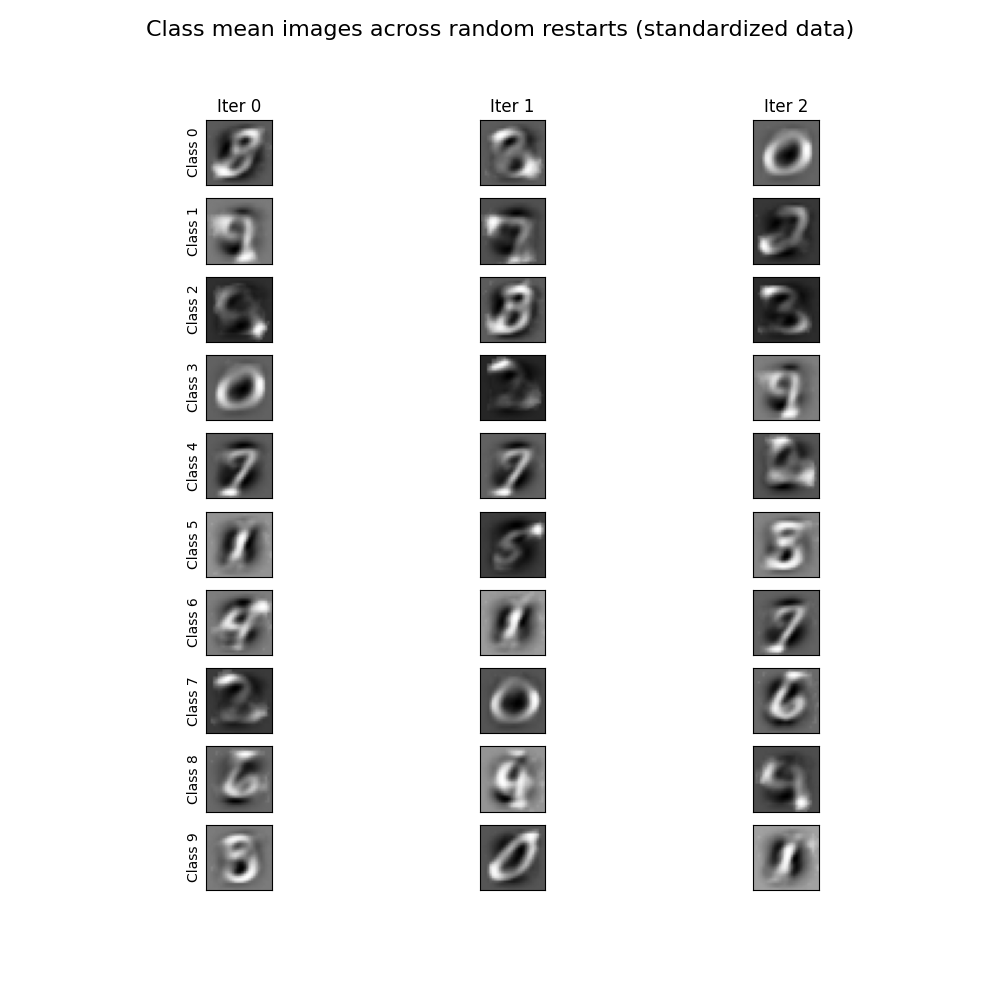
\includegraphics[width=0.85\textwidth]{p2.3.png}
\end{center}

\textbf{5.} The HAC mean images for max, min, and centroid linkage are shown below. Max linkage produces the most diverse and meaningful centroids because it tends to form compact, balanced clusters. Each centroid averages a coherent group and resembles a distinct digit prototype, though the averaging makes them somewhat soft or blurry. Both min linkage and centroid linkage suffer from chaining, one massive cluster absorbs nearly all data points while the remaining clusters are near singletons. The singleton centroids are visually the crispest (they are essentially individual images), but they do not represent meaningful class prototypes. The large cluster's centroid is a blurry average of many digit classes. Among the chained methods, centroid linkage's singletons are more diverse than min linkage's which are dominated by repeated $2$s. HAC only needs one run because it is a deterministic algorithm given a fixed linkage criterion and distance metric, there is no random initialization.

\begin{center}
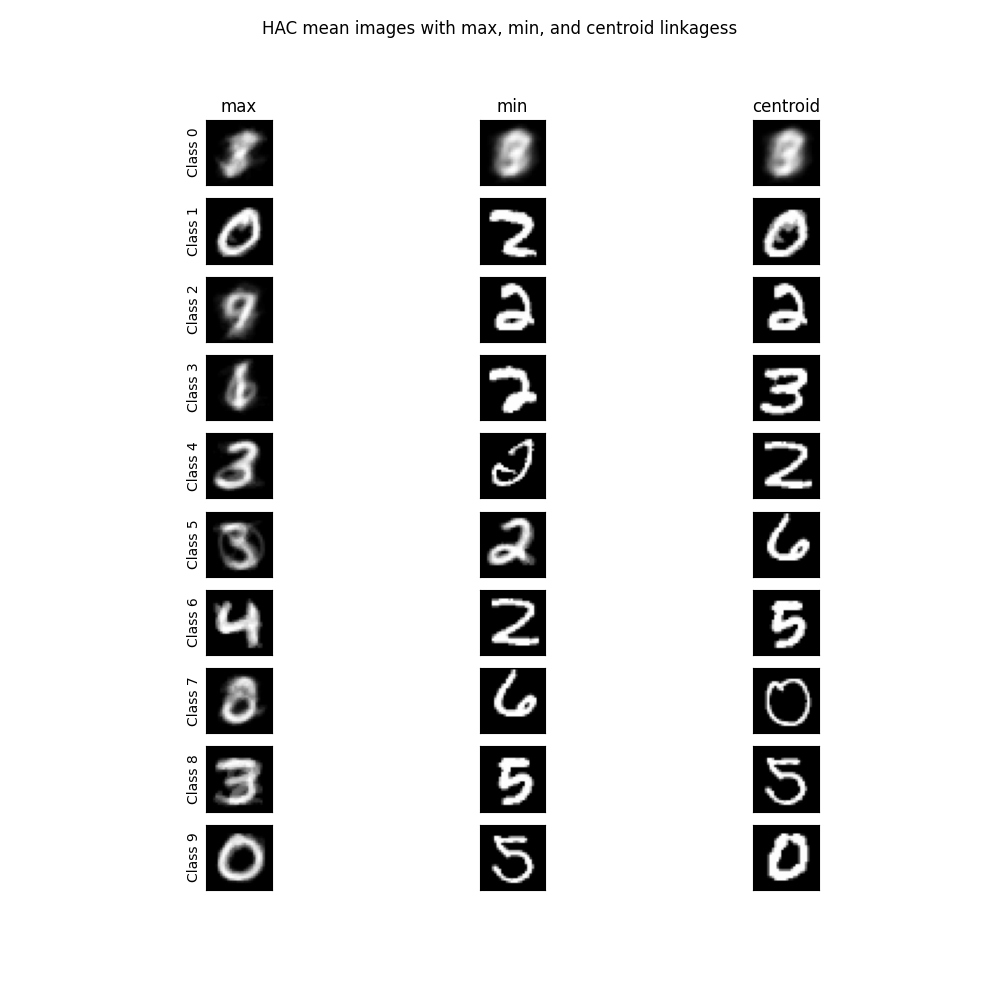
\includegraphics[width=0.85\textwidth]{p2.4.png}
\end{center}

\textbf{6.} The cluster size bar plots are shown below. Max linkage produces relatively balanced cluster sizes across the 10 clusters. Both min linkage and centroid linkage exhibit severe chaining, a single cluster absorbs nearly all of the 300 data points while the remaining clusters are near singletons. Centroid linkage is nearly as imbalanced as min linkage in this regard, not meaningfully between the two extremes. K-means produces the most balanced clusters overall since it optimizes a global objective that distributes points among centroids.

\begin{center}
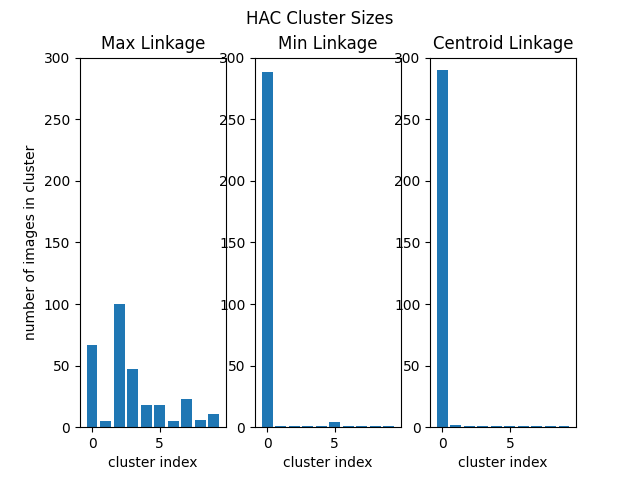
\includegraphics[width=0.85\textwidth]{p2.5a.png}
\end{center}
\begin{center}
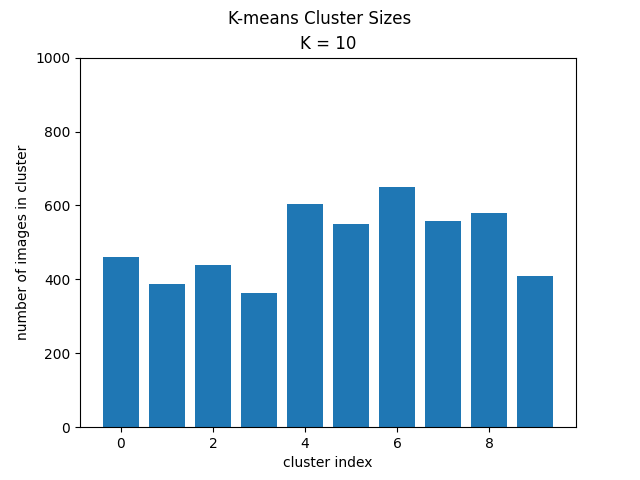
\includegraphics[width=0.5\textwidth]{p2.5b.png}
\end{center}

\textbf{7.} The pairwise confusion matrices between the clustering methods are shown below. Max linkage HAC is closest to K-means as their confusion matrix shows the most spread and structure, indicating that many K-means clusters map coherently onto max linkage clusters. This is expected since both methods produce relatively balanced partitions. In contrast, the confusion matrices involving min linkage and centroid linkage are dominated by a single row (the giant chained cluster), reflecting a partition that is structurally very different from K-means.

\begin{center}
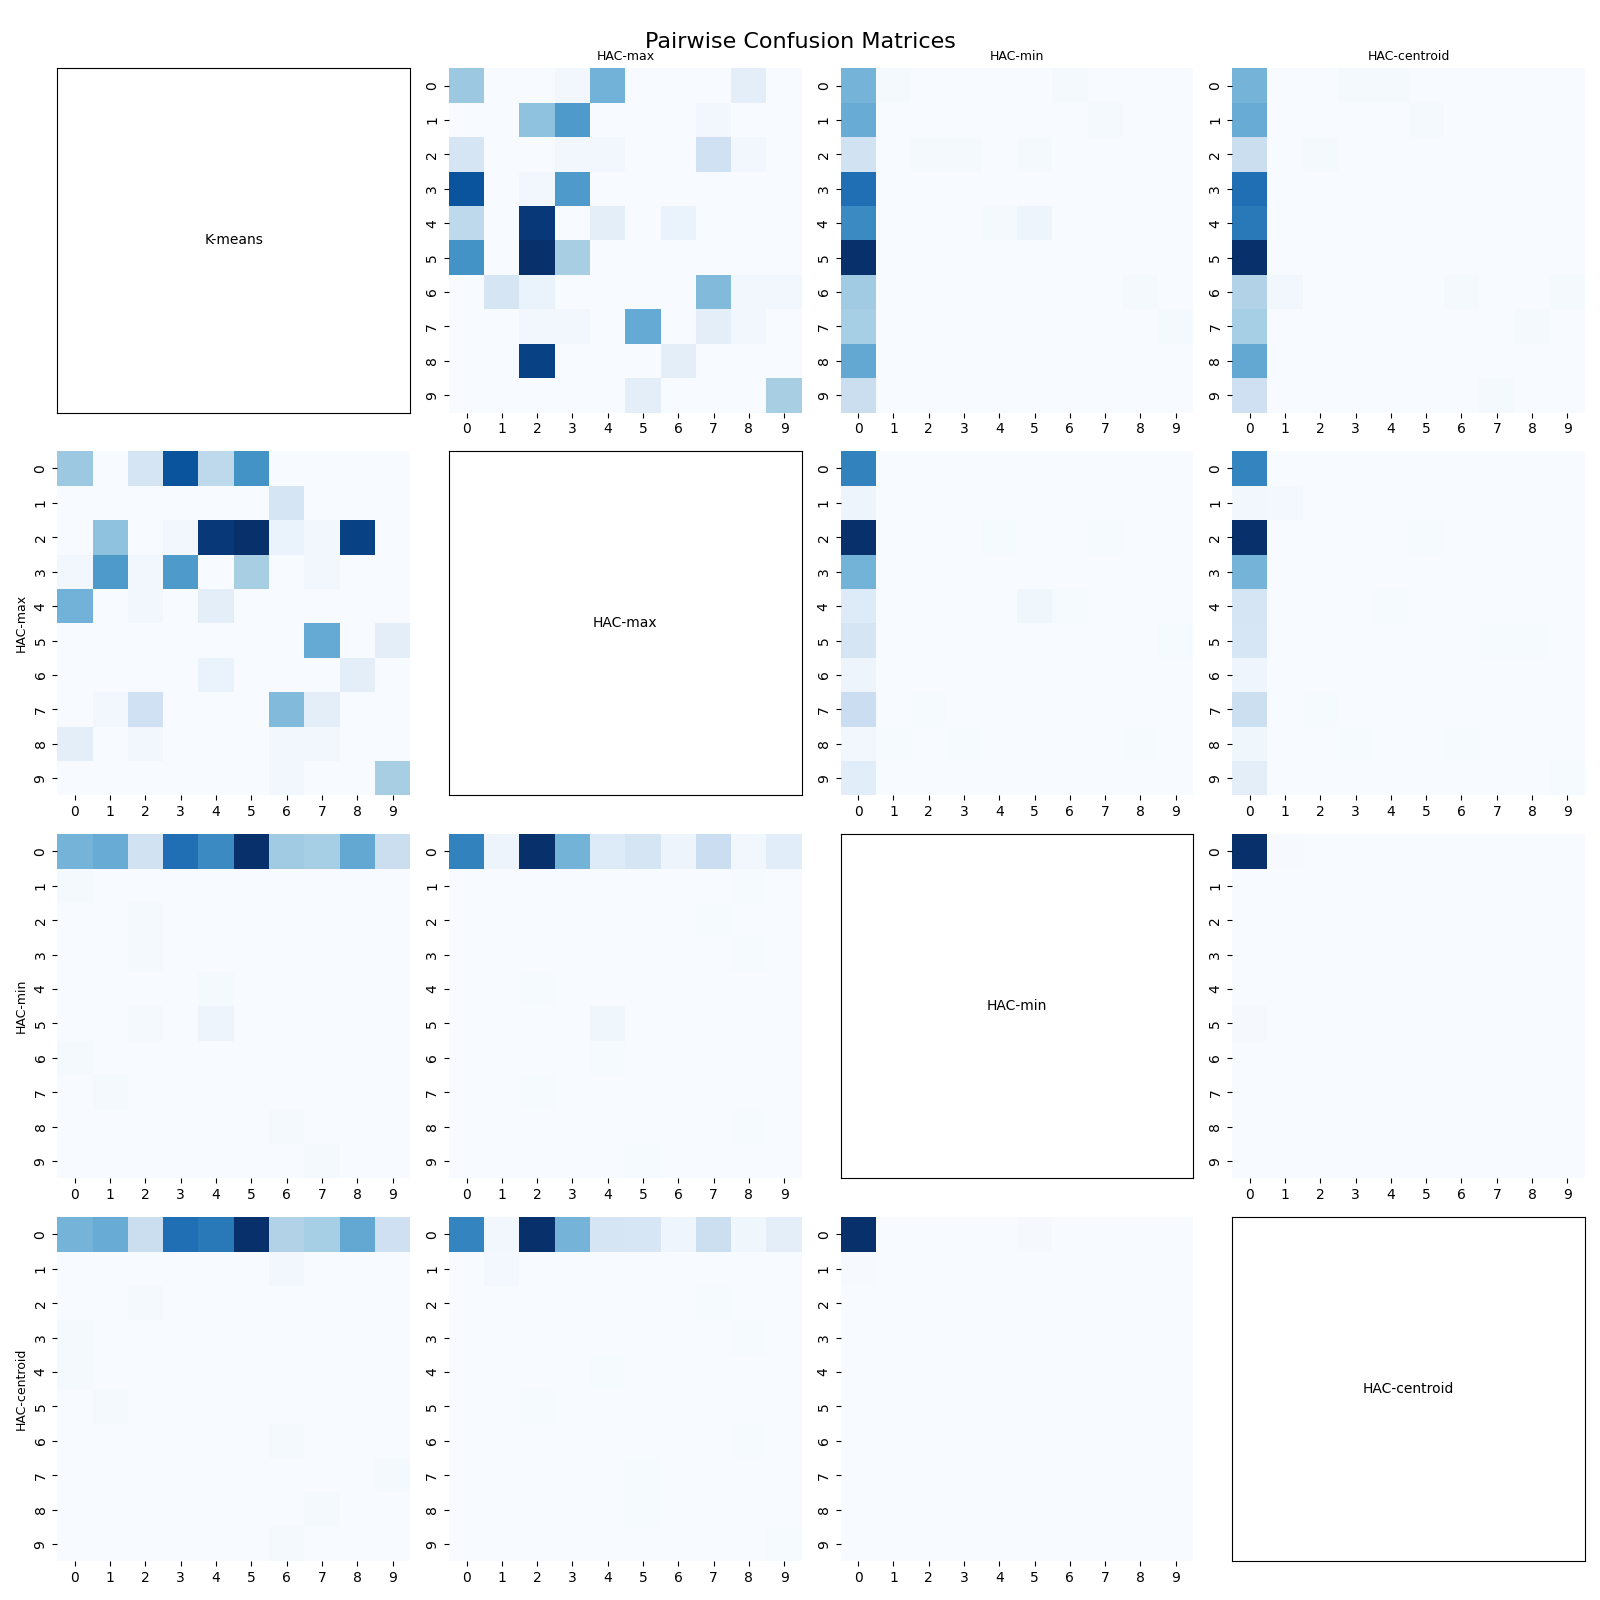
\includegraphics[width=\textwidth]{p2.6_confusion.png}
\end{center}

\textbf{8.} Clustering is a reasonable unsupervised strategy for grouping visually similar digits, but clusters should not be expected to perfectly match true labels. The algorithms group by pixel level similarity (Euclidean distance), which does not always align with semantic identity: for example, a slanted $1$ may be closer in $\ell_2$ to a $7$ than to an upright $1$. Digits with similar stroke structure (for example $3/8$, $4/9$, $7/1$) are frequently confused. Adversarial or pathological data, such as heavy noise, unusual rotations, or scaled digits, easily breaks distance based clustering because these perturbations dramatically change the pixel representation without changing the semantic class.

\end{solution}

\newpage

\begin{problem}[PCA]

  For this problem you will implement PCA from scratch on the first 6000 images of the MNIST dataset. Your job is to apply PCA on MNIST and discuss what kind of structure is found. Implement your solution in \texttt{hw5\_release.ipynb} and attach the final plots below. \\

  \noindent {\bfseries Do not use third-party PCA implementations (for example, {\normalfont \texttt{scikit-learn}}).}
  \begin{enumerate}

    \item Compute the PCA. Plot the eigenvalues corresponding to the most
    significant 500 components in order from most significant to
    least. Make another plot that describes the cumulative proportion of
    variance explained by the first $k$ most significant components for
    values of $k$ from 1 through 500.  How much variance is explained by
    the first 500 components?  Describe how the cumulative proportion of
    variance explained changes with $k$.  Include this plot below.

    \item Plot the mean image of the dataset and plot an image
    corresponding to each of the first 10 principle components.  How do
    the principle component images compare to the cluster centers from
    K-means? Discuss any similarities and differences.  Include these
    two plots below.
    
    \textit{Reminder: Center the data before performing PCA.}

    \item Compute the reconstruction error on the dataset using the first 10 principal components. Then compute the reconstruction error when the reconstruction for each point is just the mean
    image of the dataset. How do these errors compare to
    the final objective loss achieved by using K-means on the dataset?
    Discuss any similarities and differences.

    For consistency in grading, define the error function as the squared L2
    norm of the difference between the true data and the reconstruction, averaged over all data points.
  
    \item Suppose you took the original matrix of principle components
    that you found $V$ and multiplied it on the right side by some rotation matrix $R$ (i.e., you considered the matrix $VR$).
    Would that change the quality of the reconstruction error in the
    last problem?  The interpretation of the components?  Why or why
    not?

  \end{enumerate}
\end{problem}

\newpage

\begin{solution}

\textbf{1.} The eigenvalue spectrum and cumulative fraction of variance explained are plotted below. The first 500 principal components explain nearly all of the total variance (very close to 100\%). The cumulative variance curve rises steeply for the first $\sim$50 components, capturing coarse digit structure, then levels off, with diminishing returns for each additional component. This elbow shape indicates that most of the useful signal lives in a low dimensional subspace.

\begin{center}
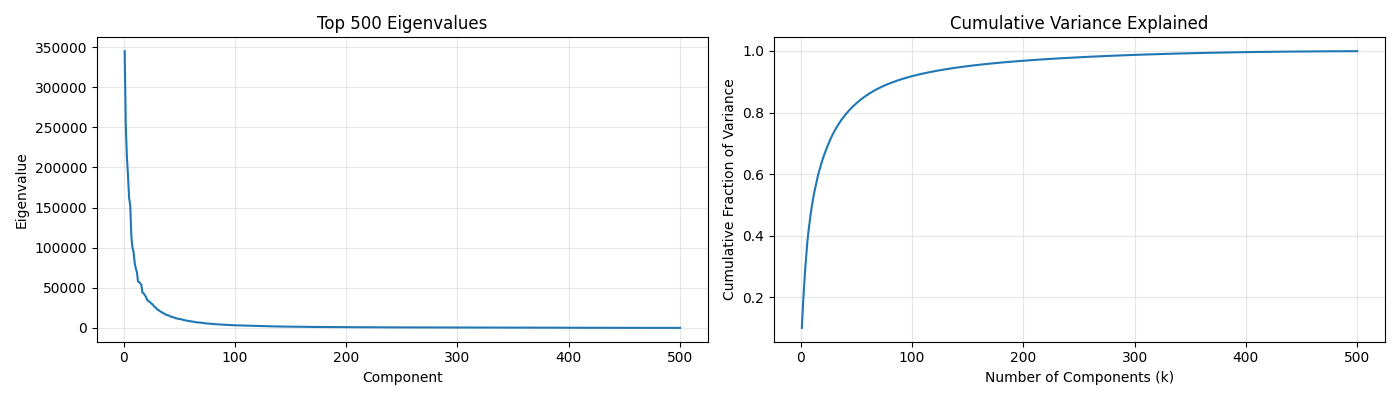
\includegraphics[width=0.85\textwidth]{pca_eigenvalues.png}
\end{center}

\textbf{2.} The mean image and the first 10 principal components are shown below. Unlike K-means centroids, which resemble individual digit prototypes (each centroid looks like a specific digit class), the principal components capture orthogonal directions of maximum variance across the entire dataset. The first few components encode global structure (overall brightness, tilt, width), while later components capture finer edge and stroke details. PCA components mix features from multiple digit classes because they are constrained to be orthogonal, whereas K-means centroids are free to each specialize to a cluster.

\begin{center}
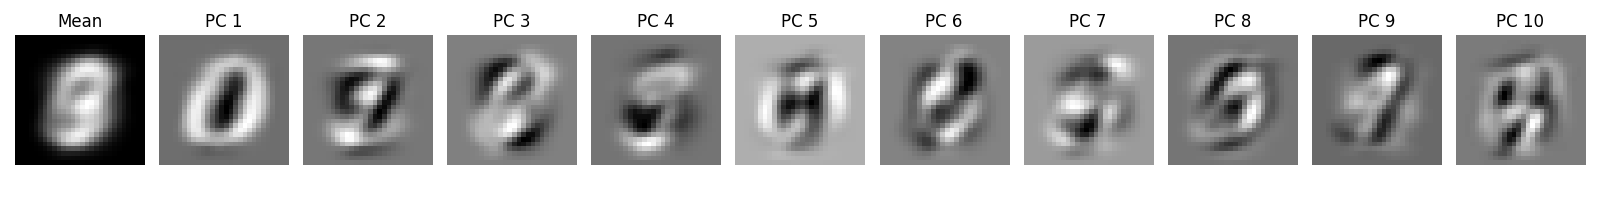
\includegraphics[width=0.85\textwidth]{pca_components.png}
\end{center}

\textbf{3.} Let the mean only reconstruction error be $E_{\mathrm{mean}} = \frac{1}{N}\sum_{i=1}^N \|x_i - \bar{x}\|_2^2$ and the PCA-10 reconstruction error be $E_{\mathrm{PCA}} = \frac{1}{N}\sum_{i=1}^N \|x_i - \hat{x}_i^{(10)}\|_2^2$, where $\hat{x}_i^{(10)}$ is the projection onto the top 10 components plus the mean. Computing these on the dataset gives:
\[
E_{\mathrm{mean}} \approx 3{,}436{,}023.25, \qquad E_{\mathrm{PCA}} \approx 1{,}731{,}315.38
\]

The PCA-10 reconstruction error is strictly less than the mean only error because projecting onto 10 components captures additional variance beyond the mean. Comparing to the K-means final objective (which is also an average squared $\ell_2$ error from each point to its cluster center with $K=10$), we see that K-means can achieve lower reconstruction error than PCA-10 because each point is reconstructed by its nearest centroid, a piecewise constant approximation, rather than a single linear subspace. However, PCA provides a globally optimal linear reconstruction in the least squares sense, and with more components it can surpass K-means.

\textbf{4.} Multiplying $V$ on the right by a rotation matrix $R$ does not change the reconstruction error. The reconstruction projects each centered point onto the column space of $V_{10}$ (the first 10 rows of $V$). Since $R$ is orthogonal, $V_{10} R$ spans the same subspace as $V_{10}$, so the projection is identical and the squared error is unchanged.

However, the interpretation of the individual components does change. The original columns of $V$ are ordered by decreasing variance and are mutually orthogonal eigenvectors of the covariance matrix. After rotation, the new columns $VR$ are still orthonormal but no longer align with the principal axes of variance, so they lose the most variance first ordering and the interpretability as independent modes of variation.

\end{solution}

\end{document}
